\section{Context}

\subsection{Introduction}

\justify
Computational science is a growing field that allows researchers to predict the behaviour of systems. For example, a physicist can write a program to predict the trajectory of a sphere instead of calculating it by hand.

\justify
 What if we bring this further?  We can try to optimize the aero-dynamism of a plane to save fuel, the behaviour of the human body cells to a recently designed drug or even given a genome figure out the risk of cancer.

\justify
Computing these are at a high cost. It is not conceivable to solve the problems on our laptops as the number of calculations and data required to process is overwhelming. To solve these tasks, we need supercomputers.

\justify
Supercomputers are machines with a huge compute power oriented to scientific and technique jobs. These machines are many small machines interconnected. Developers must write their code in a manner that the program is capable of run in parallel. 

\justify
Writing efficient parallel programs is a difficult task and even more so if the developer's specialization is not computer science. In this work, we will study and improve Alya\cite{alya}, a real use case application. In particular, we will focus on the module in charge of computing combustion processes.


\justify
This work is under an Educational Cooperation Agreement between the Facultat d'Informàtica de Barcelona and the Barcelona Supercomputing Center.

\justify
The study has been developed within a Curricular internship in the Barcelona Supercomputing Center precisely in the High-Level Support Team (HLST) inside the Operations department and developed under a Performance Optimization and Productivity\cite{popWeb} (POP) Center of Excellence Performance Analysis request.

\subsection{Terms and concepts}
\justify
In the following sections you will find basic concepts to better understand the project.

\subsubsection{High-performance computing}

\justify
High-performance computing (HPC) refers to the act of grouping compute power to do massive and complex computations and data processing. Nowadays HPC is associated to supercomputers.

\subsubsection{Supercomputer}

\justify
A supercomputer is a machine designed for HPC. The basic structure of a supercomputer consists of multiple computing nodes interconnected. Usually, a node is a shared memory system which can run programs by itself and may have add-ons like accelerators.

\subsubsection{Parallel Programming model}

\justify
Parallel programming models\cite{programminModels} add an abstraction to parallel computer architectures.  It defines constructs that allow to operate with the parallel machine performing different actions. For example, sending and receiving messages between processes, reading and writing to the shared memory or spawning tasks in form of threads, all depending on the kind of programming model.

\justify
In this section, you will find an explanation of the parallel programming models used in this work.

\subsubsection{Message Passing Interface (MPI)}

\justify
The message passing interface\cite{mpi} defines a standard  interface for communications between processes. This allows applications to run in numerous nodes. The processes use the standard interface to send messages to each other using the underlying interconnection network of the machine.  This interface allows, among other things, process synchronization, data-sharing via asynchronous and synchronous messages, gathering and scattering data, parallel input-output (I/0).

%\subsubsection{OmpSs}
%
%OmpSs is a parallel programming model that defines a set of directives and routines that allow the programmer to develop a concurrent program on a shared memory system using tasks.
%
%A task represents a unit of work, the programmer annotates its code defining tasks and dependencies between tasks. The OmpSs runtime figures out the dependency graph expressed by the programmer and tries to determine the optimal parallel execution (if possible).
%
\subsubsection{MareNostrum 4}

\justify
MareNostrum 4\cite{mn4} is a supercomputer managed by the Barcelona Supercomputing Center and managed by the Operations department. It is divided in two blocks, the general purpose block which represents the majority of the computing power and the emergent technologies block that aims to test new technologies. Figure \ref{fig:mn4} shows a picture of the supercomputer located in the "Torre Girona" chapel.

\justify
In this work we will be running the application on the general purpose block.
The general purpose block consists of 3456 nodes each node containing 2 Intel Xeon 8160 with 24 cores each running at 2.1 GHz. The interconnection network consists of an Intel Omni-Path full-fat tree at 100 Gbps.

\begin{figure}[htbp]
  \centering
  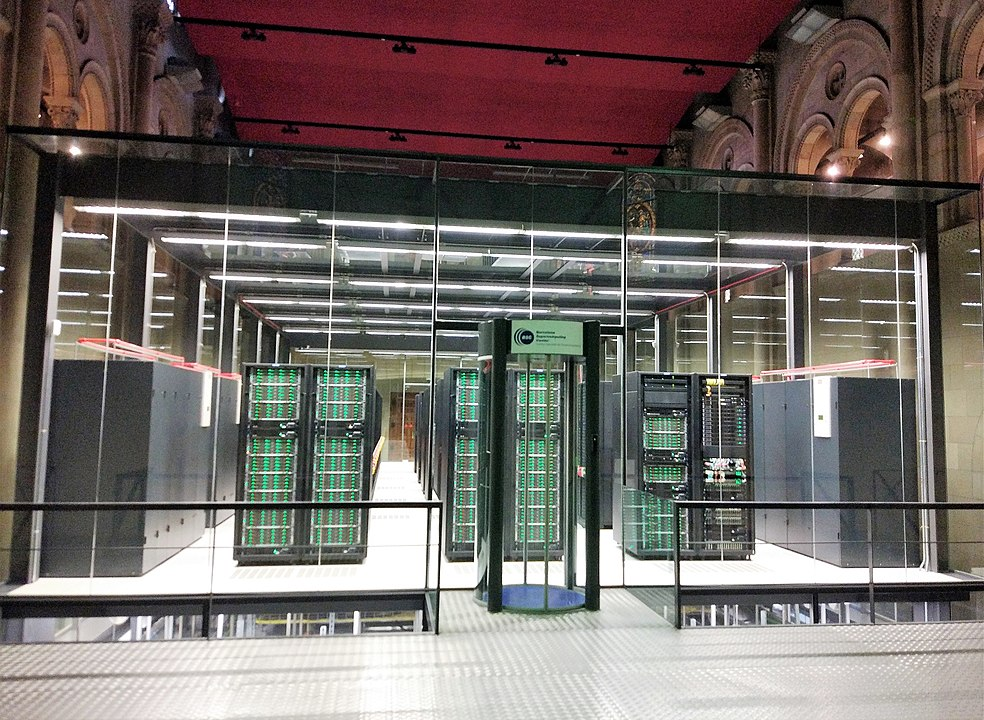
\includegraphics[width=0.6\textwidth]{mn4}
  \caption{MareNostrum 4 machine. {By Gemmaribasmaspoch - Own work, CC BY-SA 4.0, \url{https://commons.wikimedia.org/w/index.php?curid=61308843}}}
  \label{fig:mn4}
\end{figure}

\subsubsection{Alya}

\justify
Alya\cite{alya} is the application we will be studying.  It is a high-performance computational mechanics that aims to solve engineering coupled problems. In other words, Alya consists of multiple modules that can be joined to solve a specific problem. For this work, we will focalise the analysis into a new Alya module devoted to simulate combustion processes.

\justify
Alya supports a wide variety of programming models but the module we are given to analyse only supports MPI.

\subsubsection{Performance Analysis}

\justify
Running real use case scientific applications in supercomputer environments is crucial to identify flaws that deplete its performance when running on several machines.

\justify
Performance analysis refers to the process of gathering data from application executions, study the data and finally identify bottlenecks of the program.

\justify
In the state-of-the-art performance analysis, there is a wide variety of methodologies. However, this work is under the POP Center of Excellence resultantly we chose its methodology \cite{popMethod}.

\subsubsection{BSC tools}
\justify
As said, for a performance analysis we need data about the execution of programs and tools to visualize the data to get an insight of the bottlenecks.

\justify
The main BSC tools we are going to use are:

\begin{itemize}
  \item \textbf{Extrae}\cite{extraeTools}: This is the central tool of all the collection of tools. It allows the user to hook up Extrae to the application and gather data during the execution. We can trace events such as the MPI calls, PAPI\cite{papi}  counters, other programming models events and even manually instrument the code using Extrae API. All the data extracted is dumped into a file we call trace.
  \item \textbf{Basic Analysis} is a framework that given a set of traces automatically computes metrics such as POP metrics.
  \item \textbf{Paraver}\cite{paraverPaper}\cite{paraverWeb} is a desktop application that allows to load up traces and visualize the executions. Figure \ref{fig:trace} shows a trace visualization using Paraver. Y-axis displays processes, the x-axis represents time, and the colour represents what the process is doing at a certain time, in this case blue means running the application and black means not computing, either it can be idle waiting for a message or waiting for other processes or waiting for I/O... 

    \begin{figure}[htbp]
      \centering
      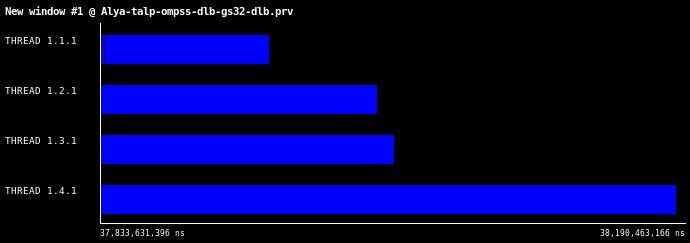
\includegraphics[width=0.6\textwidth]{sample_trace}
      \caption{Sample Paraver trace}
        \label{fig:trace}
    \end{figure}
\end{itemize}

\subsection{Problem to be resolved}
\justify
This project is motivated by the Propulsion Technologies BSC group applying to a POP Performance Analysis assessment.

\justify
The problem to solve is directly defined by the objectives in Section \ref{sec:justification}.

\subsection{Stakeholders}

\justify
The following groups will benefit from the work.

\subsubsection{Propulsion Technologies BSC group}

\justify
This is the principal stakeholder as it is the developer of the module and the applicant for the analysis.

\subsubsection{Scientific community}

\justify
This stakeholder is also benefited from the job since the results and conclusions of the study are public and open to the scientific community.
